\section{簡介}
在第\ref{ch3}章中,嘗試了直接將語音文件跟語音查詢詞編碼成向量,進行口述詞彙偵測。雖然表現不如非監督式的動態時間規劃,但至少實作出可以捨棄語音辨識系統的口述詞彙偵測。第\ref{ch3}章中,直接將語音查詢詞變成一個向量是很合理的,因為語音查詢詞只包含完整的查詢詞,並無多餘的部分,但語音文件為一整個段落,包含了許多並非查詢詞的資訊,導致產生出來的語音文件向量喪失了查詢詞的特徵。即使後面分類器在複雜,但因語音文件向量中喪失了查詢詞特徵,所以無法準確的分辨出來。本章將專注式機制引入,專注式機制可以使模型專注在某個地方,將多餘的資訊濾除。藉由專注式機制使模型能夠關注在查詢詞的部分,可以有效保留著查詢詞特徵在產生出來的語音文件向量中,則不會分心在其他非查詢詞的部分。所以本章藉由專注式機制產生出較好的語音文件向量,可以保留著查詢詞的部分,不會被其他多餘的詞彙影響,以提升口述詞彙偵測的效能。
\section{專注式機制}
專注式機制,在近年漸漸受到大家重視,專注式機制最早被應用於機器翻譯的領域上,該系統為先前\ref{seq2seq}章提到的編碼器-解碼器遞迴神經網路,能提供端對端機器翻譯。而該系統的特點為能夠根據前一個時刻的輸出,去側重當今時刻的資料中重要的部分;如此這種根據狀況進行「挑選」的技能是先前的其他類神經網路所無法比擬的。
現已出現一些模擬專注力的神經網絡架構,如記憶網絡(Memory
Network)~\cite{sukhbaatar2015end}、類神經圖靈機(Neural Turing
Machine)~\cite{graves2014neural}、 動態記憶網路(Dynamic
Memory
Network)~\cite{kumar2015ask}等等,這類模型統稱專注式模型(Attention-based
Model)。

專注式模型常應用在問答(Question
Answering,QA)系統上,讓機器可以針對提出的問題,回答正確的答案。當使用者輸入問題時,專注式模型可以幫助機器從資料庫中選擇相關資料,而將專注力放在相關的資料上,避免其他無關資訊干擾,藉此得到問題的答案。問答系統甚至已經從文字擴展到多媒體,機器可以依據圖片回答相關問題(如:圖中的人穿什麼顏色的衣服)~\cite{agrawal2015vqa},而專注式機制可以幫助模型將重心放在圖片中人的衣服上,來判斷衣服的顏色,不會受到圖片中其他物件影響。不只如此,專注式模型也被應用在自動新聞摘要~\cite{rush2015neural}、自動產生圖片/影像說明~\cite{xu2015show}、語音辨識~\cite{chan2016listen}~與機器自動翻譯等任務上~\cite{bahdanau2014neural}。

受到這些啟發,將專注式機制應用於口述詞彙偵測。在第\ref{ch3}章中,編碼器最主要的難處是當輸入序列相當長時,可能會有比較多雜訊在其中、或者許多部分是與整體資訊無關的,這些或多或少都會影響編碼出來的語音文件向量,進而影響分類器判斷結果的正確率。因此我們希望透過專注式機制的特性,建立在原本長短期記憶神經網路就能處理序列問題的基礎上,再自動從序列中挑出重要的部分並且忽略其餘跟查詢詞無關的部分,使其語音文件向量能夠包含著查詢詞的資訊,使平均準確率能夠提升。
\section{模型架構}
\subsection{系統架構簡介}
\begin{figure}[h]
\centering
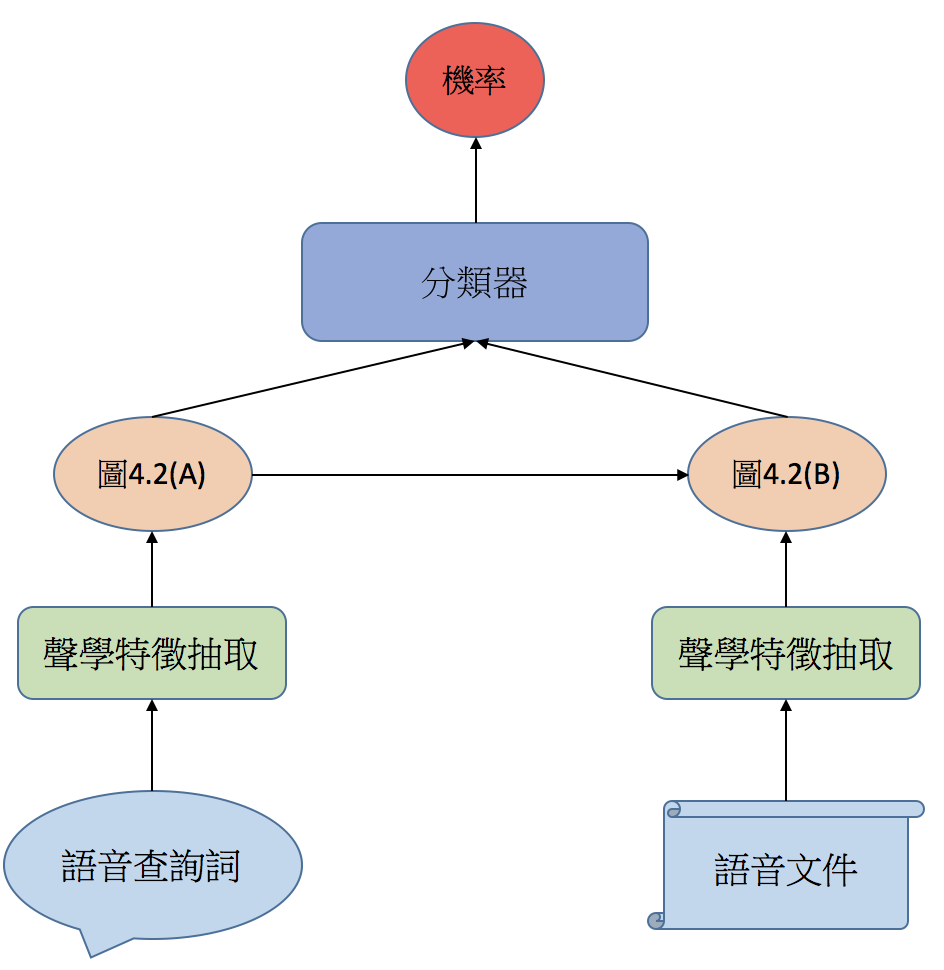
\includegraphics[scale=0.5]{images/ch4_model.png} 
\caption{模型架構圖}
\label{ch4_system}
\end{figure}
圖\ref{ch4_system}為本章節之系統架構圖。系統輸入部分包含了語音查詢詞跟語音文件,分別會經由聲學特徵抽取,轉變為39維的梅爾倒頻譜係數。首先,語音查詢詞的聲學特徵序列如同第\ref{ch3}章一樣被壓縮編碼並表示成為一向量,此向量稱之
$V_Q$ ,此部分會在\ref{ch4_query_vec}章在做介紹。產生出了 $V_Q$
,於\ref{ch4_doc_vec}章中將使用專注式機制找出跟語音查詢詞有關的部分,產生出較好的語音文件向量
$V_S$ 。最後,將 $V_Q$ 跟 $V_S$ 藉由分類器去預測查詢詞出現在文件中的機率,將在\ref{ch4_classify}章中作介紹。
\subsection{語音查詢詞之向量表示法}
\begin{figure}[h]
\centering
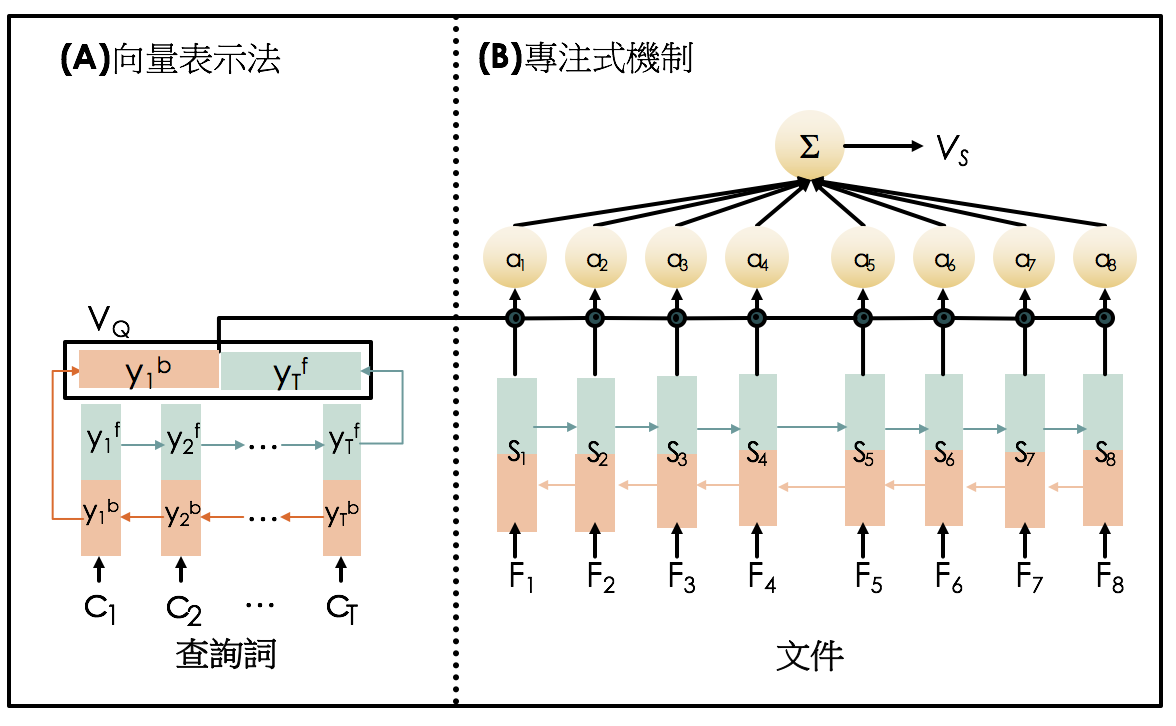
\includegraphics[scale=0.7]{images/ch4_att.png} 
\caption{專注式機制流程圖}
\label{ch4_att}
\end{figure}
\label{ch4_query_vec}
圖\ref{ch4_att}(A)為抽取 $V_Q$ 向量的介紹,將一連串的聲學特徵序列轉換為
$V_Q$ 的過程。輸入的查詢詞為
一長度T的序列,$C_1$, $C_2$,
...,$C_T$,其中 $C_i$ 均為39維梅爾倒頻譜係數。使用雙向式長短期記憶網路(Bidirectional
Long Short-term Memory
Network)作為編碼器的模型;其在輸入語音序列時,一個時間點只會讀取一個音框進去。在圖\ref{ch4_att}(A)中的第t個時間點時,正向(forward)長短期記憶網路的隱藏層輸出表示為
$y_t^f$ 、而反向(backward)長短期記憶網路之隱藏層輸出表示為 $y_{t}^b$
。在讀入所有的輸入序列之後,可在正向長短期記憶網路的最後一個時間點獲得一組隱藏層輸出向量
$y_{T}^f$ 、在反向長短期記憶網路的第一個時間點獲得 $y_{1}^b$
,並把他們串聯起來作為查詢詞的向量表示法 $V_Q$ , $V_Q
= [y_T^b || y_1^f]$ 。
\subsection{專注式機制與語音文件表示法}
在圖\ref{ch4_att}(A)中獲得查詢詞的向量表示法 $V_Q$
之後,之後將利用畫重點機制配合遞迴神經網路來對於語音文件的序列進行編碼,得到向量
$V_S$
,如圖\ref{ch4_att}(B)所示,語音文件的內容其實是一相當長的聲學特徵序列,但圖中我們簡化為八個音框,我們同樣使用雙向式長短期記憶網路來作為編碼的工具,其中在第t個時間點時,輸入詞彙的向量表示
$S_t$ 為正向長短期記憶網路與反向長短期記憶網路隱藏層輸出的串聯,$S_t
= [ y_t^f || y_t^b ]$。
接著我們引入專注式機制,來衡量查詢詞向量 $V_Q$
與語音文件內音框的關聯性高低,第 t 個時間點的語音文件向量 $S_t$
之專注式權重 $\alpha_t$ 為 $V_Q$ 與 $S_t$ 的相關程度,$\alpha_t=
S_t \odot
V_Q$,其中$\odot$表示兩向量之間的相關程度運算。相關程度的運算自己定義的,可以是簡單的歐式距離(Euclidean
Distance)、餘弦相似性(Cosine Similarity),也可使用類神經網路來計算,將兩向量丟入類神經網路去計算相關程度。
在本章中採用餘弦相似性當作相關程度,如式子\ref{cos_sim}所示:
\begin{equation}
	\label{cos_sim}
	\alpha_t = S_t \odot V_Q = \frac{S_t \cdot V_Q}{|S_t||V_Q|}
\end{equation}

接下來,對於所有的專注式權重 $\alpha_t$ 進行正規化,成為
$\hat{\alpha}_t$ ,正規化的方式有兩種。
\begin{itemize}
	\item{尖銳(Sharpening)正規化}
		
		我們將專注式權重透過軟式最大化(Softmax)之活化函數進行正規化:
		\begin{equation}
			\hat{\alpha}_t =
			\frac{exp(\alpha_t)}{\sum_{t=1}^{T} exp(\alpha_t)}
		\end{equation}
		由於可以確實降低資料的雜訊,此方式已被現存其餘專注式機制的相關研究所廣泛使用。
	\item{平滑(Smoothing)正規化}
		
		尖銳正規化偏好於注意一個點,因此一整個專注式權重集 $
		\boldsymbol{\alpha}
		= (\alpha_1,\alpha_2, ...,
		\alpha_T)$
		可能只會有某個向量 $\alpha_t$ 的權重特別高,其餘資訊皆被捨去。這樣的特性有可能降低口述詞彙偵測的表現。因此另外設計了一種正規化表示法,能夠考慮更多重要的點,此種方式也讓模型的多樣性因而增加。我們將原本算式中的指數函數改成S型函數(Sigmoid Function)$\sigma$:
		\begin{equation}
			\hat{\alpha}_t =
			\frac{\sigma(\alpha_t)}{\sum_{t=1}^{T}\sigma(\alpha_t)}
		\end{equation}

\end{itemize}

最後對於所有的語音文件向量 $S_t$
進行加權平均,使用的權重便為正規化後的專注式權重 $\hat{\alpha_t}$
,得到代表語音文件的向量 $V_S$,$V_S
= \sum_{t} \hat{\alpha_t} S_t$。
\label{ch4_doc_vec}
\subsection{分類器}
最後模型的輸出分數由分類器來決定的。分類器有很多種模型,常見的有支撐向量機(Support
Vector Machine)、類神經網路、貝氏分類器(Bayes
classifier)、決策樹(Decision
Tree)等等。在此章中,以多層類神經網路當作分類器,另外還使用語音文件向量 $V_S$
跟語音查詢詞向量 $V_Q$ 的餘弦相似度當作輸出分數為兩種產生分數的方式。
\label{ch4_classify}
\section{實驗與分析}
\section{本章總結}

